% !TEX root = task-3-2-1.tex
% Editable task bank. Append new BankTask blocks at the end of the document.
\documentclass[12pt,a4paper]{article}
\usepackage{physics-textbook}
\usepackage{graphicx,needspace}
\usetikzlibrary{decorations.pathmorphing}
\newif\ifShowSolutions
\ifdefined\TutorEdition
  \ShowSolutionstrue
\else
  \ShowSolutionsfalse % Change to \ShowSolutionstrue to display solutions.
\fi
\newcounter{banktask}
\newsavebox{\BankTaskBox}
\newcommand{\BankTaskContent}[3]{%
  \noindent\textbf{\thebanktask.}\quad #2\par
  \ifShowSolutions
    \Needspace{50mm}% Keep the solution heading with its opening text or diagram.
    #3\par
    \ifdefined\TutorEdition
      \ifcsname TutorSource#1\endcsname
        \nopagebreak\smallskip{\small\csname TutorSource#1\endcsname\par}%
      \fi
    \fi
  \fi
}
\newcommand{\BankTask}[3]{%
  \refstepcounter{banktask}\par\medskip
  \sbox{\BankTaskBox}{\begin{minipage}{\linewidth}%
    \BankTaskContent{#1}{#2}{#3}\end{minipage}}%
  \ifdim\dimexpr\ht\BankTaskBox+\dp\BankTaskBox\relax>\dimexpr\textheight-20mm\relax
    \Needspace{35mm}\BankTaskContent{#1}{#2}{#3}%
  \else
    \Needspace{\dimexpr\ht\BankTaskBox+\dp\BankTaskBox\relax}%
    \noindent\usebox{\BankTaskBox}\par
  \fi
  \medskip
}
\begin{document}
\BookSubsection{3.2.1}{Принцип суперпозиции}


% Source sdamgia-20888: https://phys-ege.sdamgia.ru/problem?id=20888
\BankTask{sdamgia-20888}{
Заряды $10$ и $16 \,\text{нКл}$ расположены на расстоянии $7 \,\text{мм}$ друг от друга. Какая сила будет действовать на заряд $2 \,\text{нКл}$, помещенный в точку, удаленную на $3 \,\text{мм}$ от меньшего заряда и на $4 \,\text{мм}$ от большего? (В мН.)\par
}{
\smallskip\noindent\textbf{Решение}\par

\begin{center}\begin{tikzpicture}[book diagram,>=stealth]
\draw(0,0)--(4,0);\foreach\x in{0,1.7,4}\draw[fill=white](\x,0)circle(.12);\node[left]at(0,0){$1$};\node[right]at(4,0){$2$};\draw[->,thick](1.7,0)--(.7,0)node[above]{$\vec F_2$};\draw[->,thick](1.7,0)--(2.9,0)node[above]{$\vec F_1$};\draw[<->](0,.65)--(4,.65)node[midway,above]{$7\,\text{мм}$};\draw[<->](0,-.65)--(1.7,-.65)node[midway,below]{$r_1=3\,\text{мм}$};\draw[<->](1.7,-.65)--(4,-.65)node[midway,below]{$r_2=4\,\text{мм}$};
\end{tikzpicture}\end{center}
\par
Все заряды будут находиться на одной линии, так как $3$ + $4=7$.\par
Искомая сила определяется выражением $F=F_{1} - F_{2}.$\par
Из закона Кулона:\par
\[F=k \frac{ |q_{1}| \cdot |q_{2}|}{ r ^2 } ;\]
\[F=k \frac{ |q_{1}| \cdot |q_{3}|}{ r_{1} ^2 } - k \frac{ |q_{2}| \cdot |q_{3}|}{ r_{2} ^2 } =k|q_{3}| ( \frac{ |q_{1}|}{ r_{1} ^2 } - \frac{ |q_{2}|}{ r_{2} ^2 } ) ;\]
\[F=9 \cdot 10 ^{9} \,\text{Н} \cdot \,\text{м} ^2 /\,\text{Кл} ^2 \cdot 2 \cdot 10 ^{ - 9 } \,\text{Кл} ( \frac{ 10 \cdot 10 ^{ - 9 } \,\text{Кл}}{ ( 3 \cdot 10 ^{ - 3 } \,\text{м} ) ^2 } - \frac{ 16 \cdot 10 ^{ - 9 } \,\text{Кл}}{ ( 4 \cdot 10 ^{ - 3 } \,\text{м} ) ^2 } ) =2\,\text{мН}.\]
Ответ: $2$.\par
}

% Source sdamgia-6823: https://phys-ege.sdamgia.ru/problem?id=6823
\BankTask{sdamgia-6823}{
Два точечных заряда — отрицательный, равный по модулю $3 \,\text{мкКл}$, и положительный, равный по модулю $4 \,\text{мкКл}$, расположены на расстоянии $1 \,\text{м}$ друг от друга. На расстоянии $1$ метр от каждого из этих зарядов помещают положительный заряд $Q$, модуль которого равен $2 \,\text{мкКл}$. Определите модуль силы, действующей на заряд $Q$ со стороны двух других зарядов. (В мН и округлите до целого числа.)\par
}{
\smallskip\noindent\textbf{Решение}\par

\begin{center}\begin{tikzpicture}[book diagram,>=stealth]
\coordinate(A)at(-1.5,2.6);\coordinate(B)at(1.5,2.6);\coordinate(Q)at(0,0);\draw(A)--(B)--(Q)--cycle;\fill(A)circle(1.5pt)node[above]{$-Q_1$};\fill(B)circle(1.5pt)node[above]{$+Q_2$};\fill(Q)circle(1.5pt)node[right]{$+Q$};\draw[->,thick](Q)--(-.6,1.04)node[left]{$\vec F_1$};\draw[->,thick](Q)--(-.8,-1.39)node[below]{$\vec F_2$};\draw(-.6,1.04)--(-1.4,-.35)--(-.8,-1.39);\draw[->,thick](Q)--(-1.4,-.35)node[left]{$\vec F$};
\end{tikzpicture}\end{center}
\par
Пусть $Q_{1}, Q_{2}$ — соответственно первый и второй заряды, изобразим силы, действующие на заряд $Q$ и найдем их равнодействующую (см. рис.). Заметим, что заряды лежат в вершинах равностороннего треугольника, поэтому угол между силами $\vec{F}_{1}$ и $\vec{F}_{2}$ равен $120$°. Рассмотрим треугольник $QF_{1}F,$ в нем $\angle QF_{1}F=60 ^\circ.$ Найдем модуль равнодействующей силы, используя теорему косинусов для этого треугольника:\par
\[\begin{aligned}F&=\sqrt{F_1^2+F_2^2-2F_1F_2\cos60^\circ}\\&=\sqrt{\left(k\frac{Q_1Q}{r_1^2}\right)^2+\left(k\frac{Q_2Q}{r_2^2}\right)^2-2k\frac{Q_1Q}{r_1^2}\cdot k\frac{Q_2Q}{r_2^2}\cdot\frac12}.\end{aligned}\]
По условию задачи $r_{1}=r_{2},$ поэтому:\par
\[F=k\frac{Q}{r^2}\sqrt{Q_1^2+Q_2^2-2\cdot\frac12Q_1Q_2}=\]
\[\begin{aligned}&=9\cdot10^9\frac{\text{Н}\cdot\text{м}^2}{\text{Кл}^2}\cdot\frac{2\cdot10^{-6}\,\text{Кл}}{(1\,\text{м})^2}\sqrt{\left(9+16-2\cdot\frac12\cdot3\cdot4\right)\cdot10^{-12}\,\text{Кл}^2}\\&\approx65\cdot10^{-3}\,\text{Н}=65\,\text{мН}.\end{aligned}\]
Ответ: $65$.\par
}

% Source sdamgia-7859: https://phys-ege.sdamgia.ru/problem?id=7859
\BankTask{sdamgia-7859}{
В трех вершинах квадрата размещены точечные заряды: $-q,$ +$q$, $- q$ ($q>0$) (см. рис.). Куда направлена кулоновская сила, действующая со стороны этих зарядов на точечный заряд $+2q$, находящийся в центре квадрата?\par

\begin{center}\begin{tikzpicture}[book diagram,>=stealth]
\draw(0,0)rectangle(2,2);\fill(0,0)circle(1.5pt)node[below left]{$+q$};\fill(0,2)circle(1.5pt)node[above left]{$-q$};\fill(2,0)circle(1.5pt)node[below right]{$-q$};\fill(1,1)circle(1.5pt)node[below]{$+2q$};
\end{tikzpicture}\end{center}
\par
\begin{center}\begin{tabular}{cc}1) $\rightarrow$ & 2) $\swarrow$\\3) $\nearrow$ & 4) $\nwarrow$\end{tabular}\end{center}\par
}{
\smallskip\noindent\textbf{Решение}\par
Силы притяжения со стороны отрицательных зарядов уравновешивают друг друга, поэтому суммарная сила трех зарядов совпадает с силой со стороны положительного заряда, который отталкивает центральный заряд по прямой их соединяющей, то есть вправо вверх.\par
Правильный ответ указан под номером $3$.\par
}

% Source sdamgia-39257: https://phys-ege.sdamgia.ru/problem?id=39257
\BankTask{sdamgia-39257}{
Две маленькие бусинки, закреплённые в точках А и В, несут на себе заряды $-3q$ и $+1{,}5q>0$ соответственно (см. рис.).\par
$1$) Если бусинки соединить незаряженной стеклянной палочкой, их заряды станут равными.\par
$2$) Если бусинки соединить тонкой медной проволокой, то они будут притягивать друг друга.\par
$3$) Модуль силы Кулона, действующей на бусинку В, равен модулю силы Кулона, действующей на бусинку А.\par
$4$) На бусинку А со стороны бусинки В действует сила Кулона, направленная горизонтально вправо.\par
$5$) Напряжённость результирующего электростатического поля в точке С направлена горизонтально вправо.\par

\begin{center}\begin{tikzpicture}[book diagram,>=stealth]
\draw(0,0)--(4,0);\fill(0,0)circle(2pt)node[below]{$A$}node[above]{$-3q$};\fill(2,0)circle(2pt)node[below]{$C$};\fill(4,0)circle(2pt)node[below]{$B$}node[above]{$+1{,}5q$};
\end{tikzpicture}\end{center}
\par
}{
\smallskip\noindent\textbf{Решение}\par
$1$) Неверно. Стекло является диэлектриком, поэтому при соединении бусинок стеклянной палочкой их заряды не изменятся.\par
$2$) Неверно. Медь относится к проводникам, поэтому при соединении бусинок медной проволокой их заряды станут равными по модулю и по закону сохранения заряда\par
\[q= \frac{ q_{1} + q_{2}}{ 2 } = \frac{ - 3q + 1{,}5q}{ 2 } = - 0{,}75q.\]
Такие одноименно заряженные бусинки будут отталкиваться.\par
$3$) Верно. По третьему закону Ньютона силы взаимодействия зарядов равны по модулю.\par
$4$) Верно. Заряды бусинок разноименные, поэтому они притягиваются. Следовательно, на бусинку А со стороны бусинки В действует сила Кулона, направленная горизонтально вправо.\par
$5$) Неверно. Вектор напряженности $\vec{E}_{A}$ поля, созданного бусинкой А, направлен влево. Вектор напряженности $\vec{E}_{\text{В}}$ поля, созданного бусинкой В, направлен влево. По принципу суперпозиции полей результирующий вектор $\vec{E}=\vec{E}_{A} + \vec{E}_{B}$ направлен влево.\par
Ответ: $34$.\par
}


% Source 6668: https://phys-ege.sdamgia.ru/problem?id=6668
\BankTask{6668}{
На горизонтальной плоскости в вершинах правильного пятиугольника закреплены $5$ одинаковых положительных зарядов Q  =  $1$ мкКл, расположенные на расстоянии R  =  $2\,\text{м}$ от центра этого пятиугольника. На вертикальной прямой, проведенной из этого центра, на высоте $0{,}75$R над плоскостью находится положительный заряд q  =  $4$ мкКл. Найдите модуль и направление силы F, действующей на него со стороны остальных зарядов.
}{
\smallskip\noindent\textbf{Решение}\par
По закону Кулона сила f взаимодействия зарядов Q и q, находящихся на расстоянии r друг от друга, равна $f= \frac{1}{4 \pi \varepsilon_0} \cdot \frac{qQ}{r ^2} ,$ или в векторной форме: $\vec{f}= \frac{1}{4 \pi \varepsilon_0} \cdot \frac{qQ}{r ^3} \vec{r}.$
В нашем случае $r= \sqrt{R ^2 + 0{,}75 ^2 R ^2} =1{,}25R,f= \frac{1}{4 \pi \varepsilon_0} \cdot \frac{qQ}{1{,}5625R ^2} .$ Вектор $\vec{f}$ образует с вертикалью угол $\alpha$ такой, что $\cos \alpha = \frac{0{,}75R}{1{,}25R} =0{,}6.$
Проекции всех пяти векторов $\vec{f}$ на вертикальную ось одинаковы и равны $f_\parallel= \frac{1}{4 \pi \varepsilon_0} \cdot \frac{qQ}{r ^2} \cos \alpha ,$ а их проекции на направления, перпендикулярные оси, равны $f_\perp= \frac{1}{4 \pi \varepsilon_0} \cdot \frac{qQ}{r ^2} \sin \alpha .$
В соответствии с принципом суперпозиции сил сумма пяти одинаковых векторов $\vec{f}_\perp,$ образующих правильный пятиугольник, равна нулю, а сумма пяти одинаковых векторов $\vec{f}_\parallel,$ направленных вдоль оси, дает действующую на заряд q суммарную силу, равную по модулю:

\[F= \frac{1}{4 \pi \varepsilon_0} \cdot \frac{5 \cdot 0{,}6 \cdot qQ}{1{,}5625R ^2} = \frac{1{,}92}{4 \pi \varepsilon_0} \cdot \frac{qQ}{R ^2} =17{,}28\,\text{мН}\]

и направленную вдоль оси пятиугольника «от него».

Ответ: Сила направлена вдоль оси пятиугольника «от него» и по модулю равна $F= \frac{1{,}92}{4 \pi \varepsilon_0} \cdot \frac{qQ}{R ^2} =17{,}28\,\text{мН}.$
}

% Source 30002: https://phys-ege.sdamgia.ru/problem?id=30002
\BankTask{30002}{
\begin{center}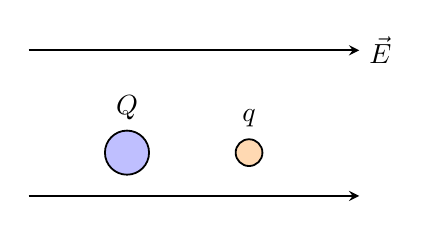
\begin{tikzpicture}[>=stealth,line width=.65pt]\draw[->](0,1.3)--(4.2,1.3)node[right]{$\vec E$};\draw[->](0,-.55)--(4.2,-.55);\draw[fill=blue!25](1.25,0)circle(.28)node[above=.29cm]{$Q$};\draw[fill=orange!30](2.8,0)circle(.17)node[above=.2cm]{$q$};\end{tikzpicture}\end{center}

В однородном электрическом поле с напряженностью E  =  $18\,\text{В}$/м находятся два точечных заряда: Q  =  -$1\,\text{нКл}$ и $q= + 5$ нКл с массами M  =  $5\,\text{г}$ и m  =  $10\,\text{г}$ соответственно (см. рисунок). На каком расстоянии d друг от друга находятся заряды, если их ускорения совпадают по величине и направлению? Сделайте рисунок с указанием всех сил, действующих на заряды. Силой тяжести пренебречь.
}{
\smallskip\noindent\textbf{Решение}\par
\begin{center}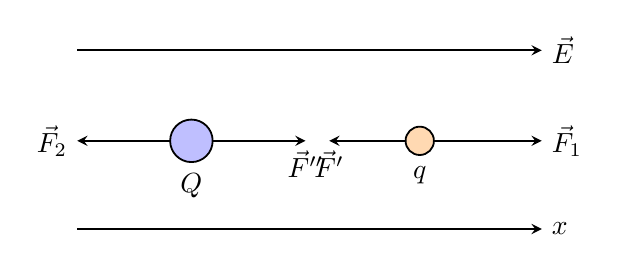
\begin{tikzpicture}[>=stealth,line width=.65pt]\draw[->](0,1.15)--(5.9,1.15)node[right]{$\vec E$};\draw[->](0,-1.12)--(5.9,-1.12)node[right]{$x$};\draw[fill=blue!25](1.45,0)circle(.27)node[below=.29cm]{$Q$};\draw[fill=orange!30](4.35,0)circle(.18)node[below=.2cm]{$q$};\draw[->](1.18,0)--(0,0)node[left]{$\vec F_2$};\draw[->](1.72,0)--(2.9,0)node[below]{$\vec F^{\prime\prime}$};\draw[->](4.17,0)--(3.2,0)node[below]{$\vec F^{\prime}$};\draw[->](4.53,0)--(5.9,0)node[right]{$\vec F_1$};\end{tikzpicture}\end{center}

$1$.  Направим ось Ox по напряженности электрического поля $\vec{E}.$ На заряд q действуют две электрические силы: $F_1=q E$ со стороны однородного поля и сила Кулона $F ^{ \prime } =F= \frac{k q|Q|}{d ^2}$ со стороны другого заряда. На заряд Q действуют сила $F_2=|Q| E$ со стороны однородного поля и сила Кулона $F ^{ \prime \prime } =F= \frac{k q|Q|}{d ^2}$ со стороны заряда q. 
$2$.  В соответствии со вторым законом Ньютона в проекциях на ось Ox имеем: 

$m a=F_1 - F, \qquad ( 1 )$ $M a= - F_2 + F.\qquad ( 2 )$

 Тогда из соотношений ($1$) и ($2$) и условия задачи получим: 

\[\frac{F_1 - F}{m} = \frac{F - F_2}{M} . \qquad ( 3 )\]

$3$.  Подставляя в ($3$) выражения для электрических сил, получим: 

\[d=\sqrt{\frac{kq|Q|(m+M)}{E(m|Q|+qM)}}=\sqrt{\frac{9\cdot10^9\cdot5\cdot10^{-9}\cdot1\cdot10^{-9}\cdot(0{,}01+0{,}005)}{18(0{,}01\cdot1\cdot10^{-9}+0{,}005\cdot5\cdot10^{-9})}}\approx1\,\text{м}.\]

Ответ: $d \approx 1 \,\text{м}.$
}

\end{document}
